%%%%%%%%%%%%%%%%%%%%%%%%%%%%%%%%%%%%%%%%%
% Simple Sectioned Essay Template
% LaTeX Template
%
% This template has been downloaded from:
% http://www.latextemplates.com
%
% Note:
% The \lipsum[#] commands throughout this template generate dummy text
% to fill the template out. These commands should all be removed when 
% writing essay content.
%
%%%%%%%%%%%%%%%%%%%%%%%%%%%%%%%%%%%%%%%%%

%----------------------------------------------------------------------------------------
%	PACKAGES AND OTHER DOCUMENT CONFIGURATIONS
%----------------------------------------------------------------------------------------

\documentclass[12pt, spanish]{article} % Default font size is 12pt, it can be changed here

\usepackage{geometry} % Required to change the page size to A4
\geometry{a4paper} % Set the page size to be A4 as opposed to the default US Letter

\usepackage{graphicx} % Required for including pictures

\usepackage{adjustbox}

\usepackage{float} % Allows putting an [H] in \begin{figure} to specify the exact location of the figure
\usepackage{wrapfig} % Allows in-line images such as the example fish picture

\usepackage{lipsum} % Used for inserting dummy 'Lorem ipsum' text into the template

\usepackage[spanish]{babel}
\selectlanguage{spanish}

\usepackage[utf8]{inputenc}

\usepackage{enumitem}% http://ctan.org/pkg/enumitem

\linespread{1.2} % Line spacing

\setlength{\parindent}{2em}
\setlength{\parskip}{1em}

%\setlength\parindent{0pt} % Uncomment to remove all indentation from paragraphs

\graphicspath{{img/}} % Specifies the directory where pictures are stored

\usepackage{concmath}
\usepackage[T1]{fontenc}

\newlist{steps}{enumerate}{1}%
\setlist[steps]{label={\arabic*)}}%

\begin{document}


\begin{titlepage}

\newcommand{\HRule}{\rule{\linewidth}{0.5mm}} % Defines a new command for the horizontal lines, change thickness here

\center % Center everything on the page

\textsc{\LARGE ammana.es}\\[1.5cm] % Name of your university/college
\textsc{\Large }\\[0.5cm] % Major heading such as course name
\textsc{\large }\\[0.5cm] % Minor heading such as course title

\HRule \\[0.4cm]
{ \huge \bfseries Manual del administrador}\\[0.4cm] % Title of your document
\HRule \\[1.5cm]

{\large \today}\\[3cm] % Date, change the \today to a set date if you want to be precise

%\includegraphics{Logo}\\[1cm] % Include a department/university logo - this will require the graphicx package

\vfill % Fill the rest of the page with whitespace

\end{titlepage}

%----------------------------------------------------------------------------------------
\tableofcontents % Include a table of contents

\newpage % Begins the essay on a new page instead of on the same page as the table of contents 

%----------------------------------------------------------------------------------------
\section{Introducción}

\textbf{ammana.es} funciona de forma prácticamente autónoma y los clientes pueden
comprar y descargar protocolos sin intervención del administrador. La única
excepción es cuando algún cliente paga por transferencia bancaria, en cuyo
caso el pago debe ser marcado como cobrado de forma manual para que el cliente
pueda descargarse el protocolo.

Por otro lado, el panel de administración de \textbf{ammana.es}, junto con los de \textbf{Paypal} y
\textbf{Quaderno}, dan acceso al administrador a la lista de clientes, facturas, pedidos, etc
para su consulta, bien por curiosidad bien para ofrecer soporte a un cliente..

Es decir, las funciones del administrador son 2:

\begin{steps}
  \item Marcar como cobrados los pedidos que han sido pagados por transferencia
  \item Acceder a la información de clientes y facturas
\end{steps}


%----------------------------------------------------------------------------------------
\section{Acceso al panel de administración}

Para acceder al panel de administración, simplemente debes hacer login con las credenciales
del usuario, administrador. Es decir:

\begin{steps}
    \item Click en ``Identificarse'':

        \medskip
        \begin{minipage}[t]{\linewidth}
        \raggedright
        \adjustbox{valign=t}{%
            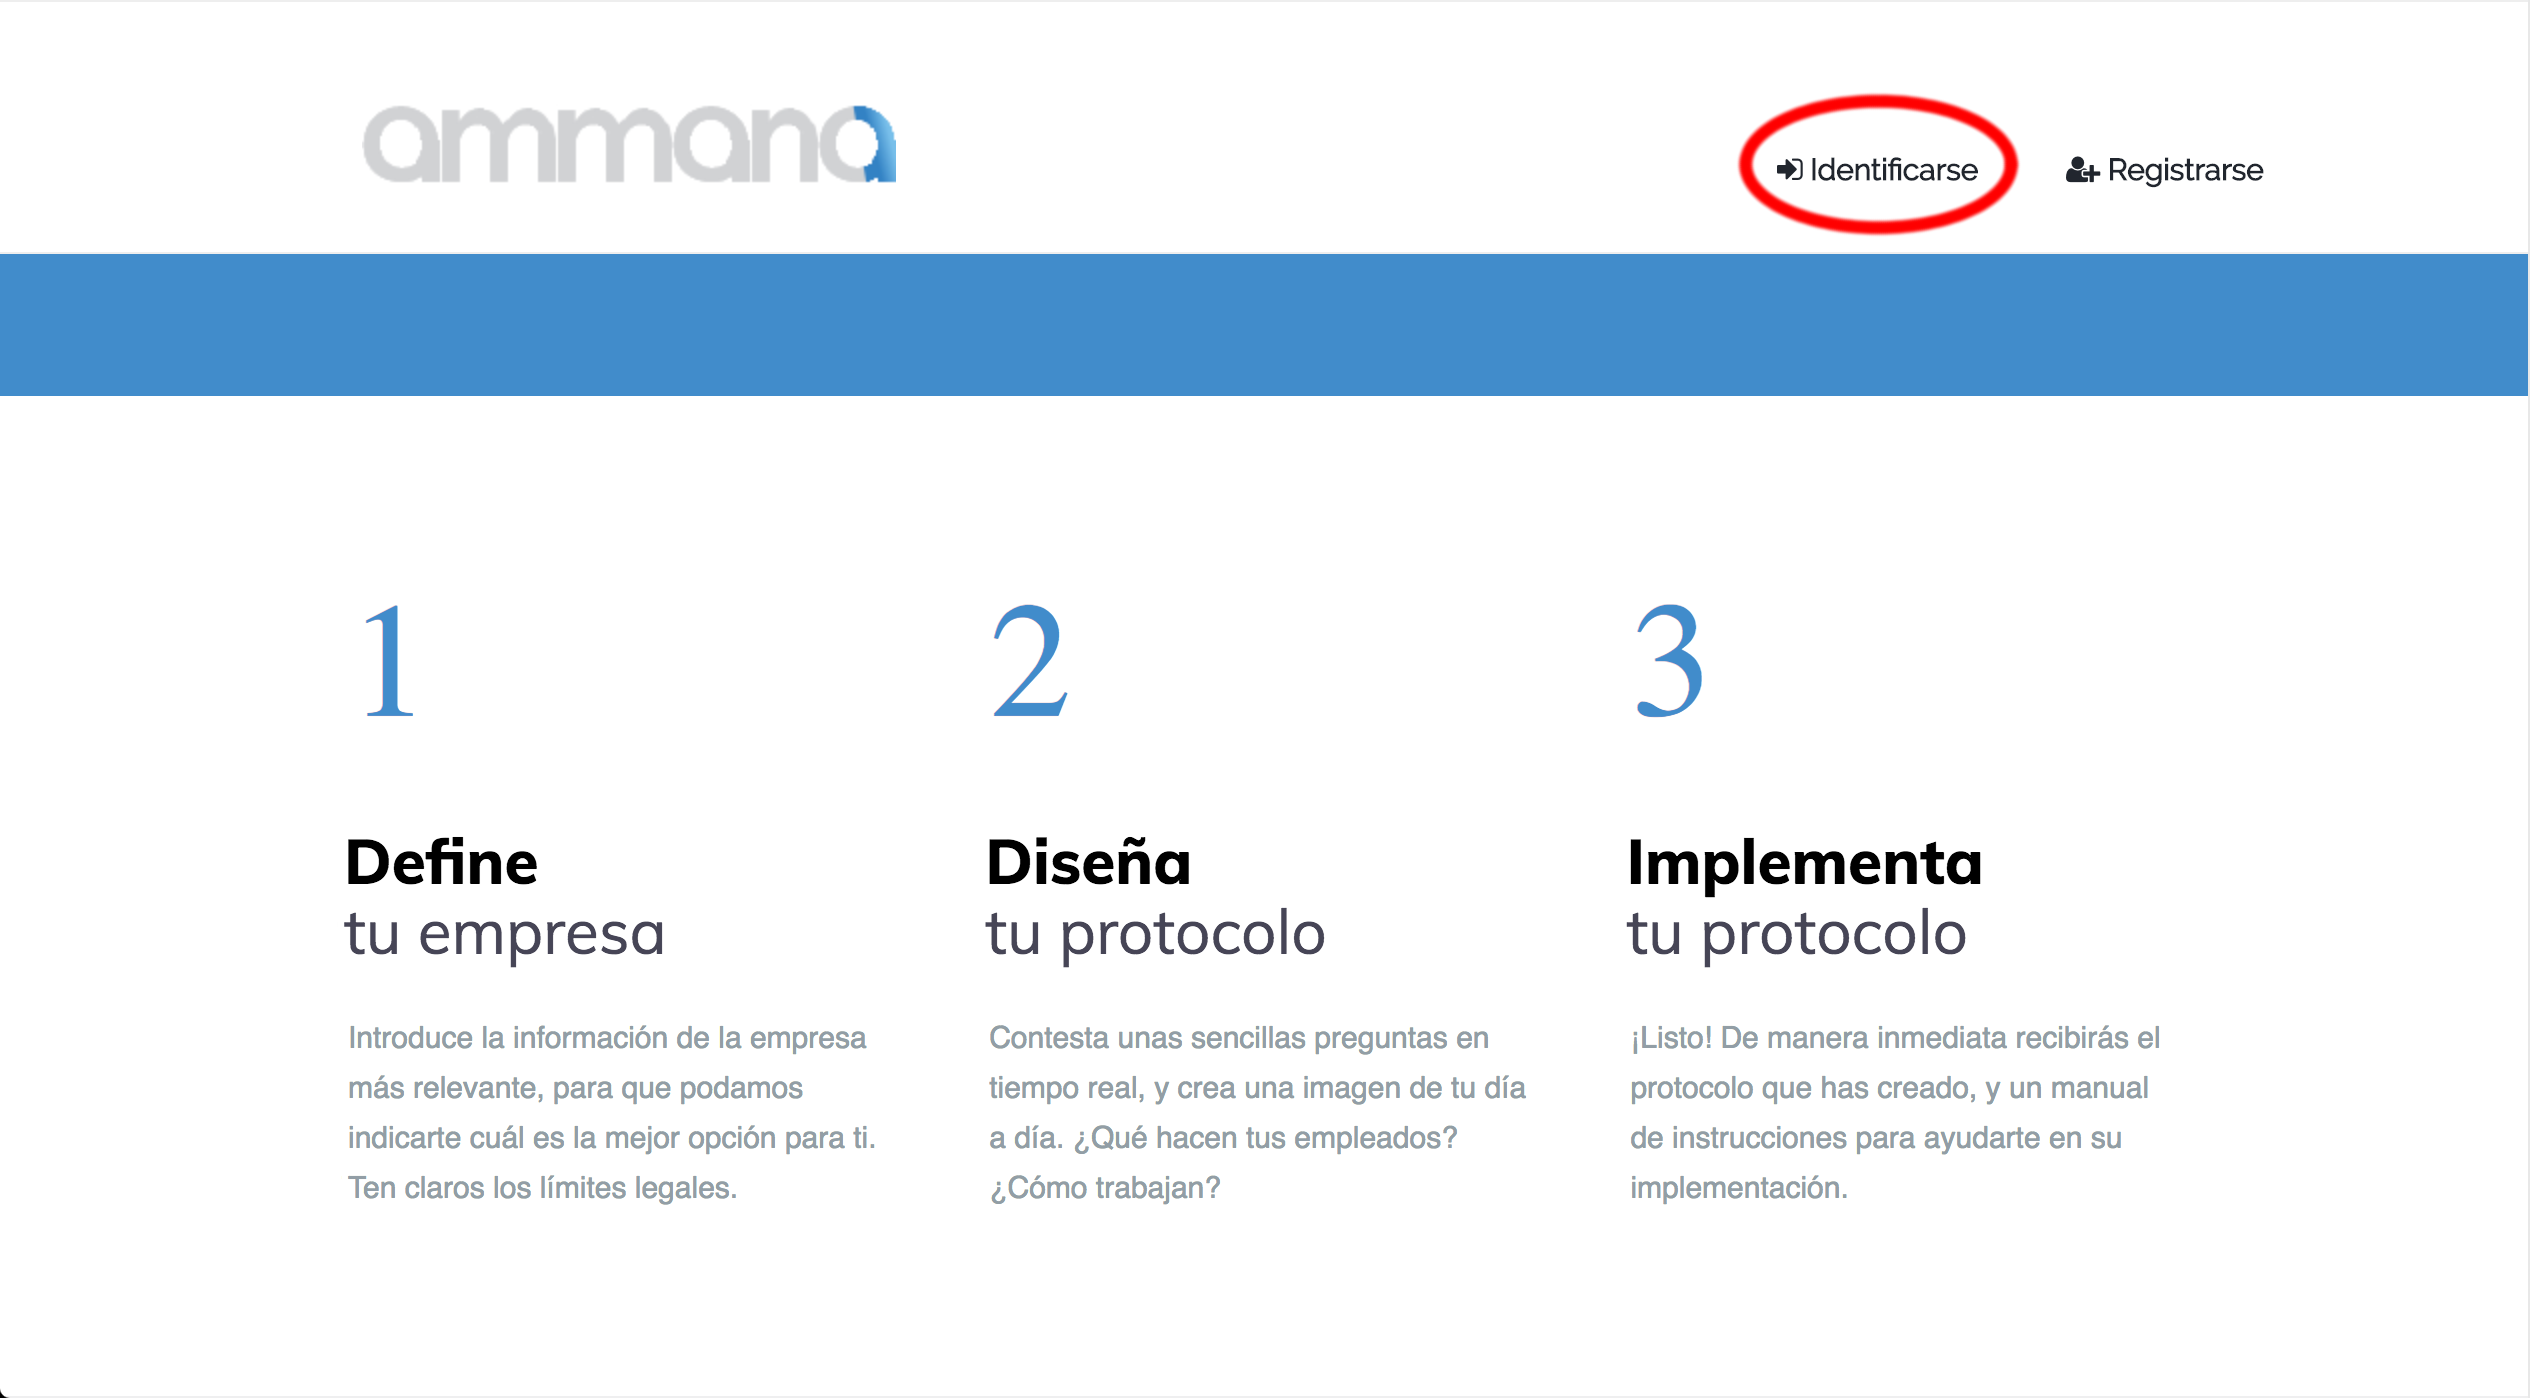
\includegraphics[width=1\linewidth]{login_button.png}%
        }
    \end{minipage}
    \item Introducir email y contraseña en el formulario de login:

        \medskip
        \begin{minipage}[t]{\linewidth}
        \raggedright
        \adjustbox{valign=t}{%
            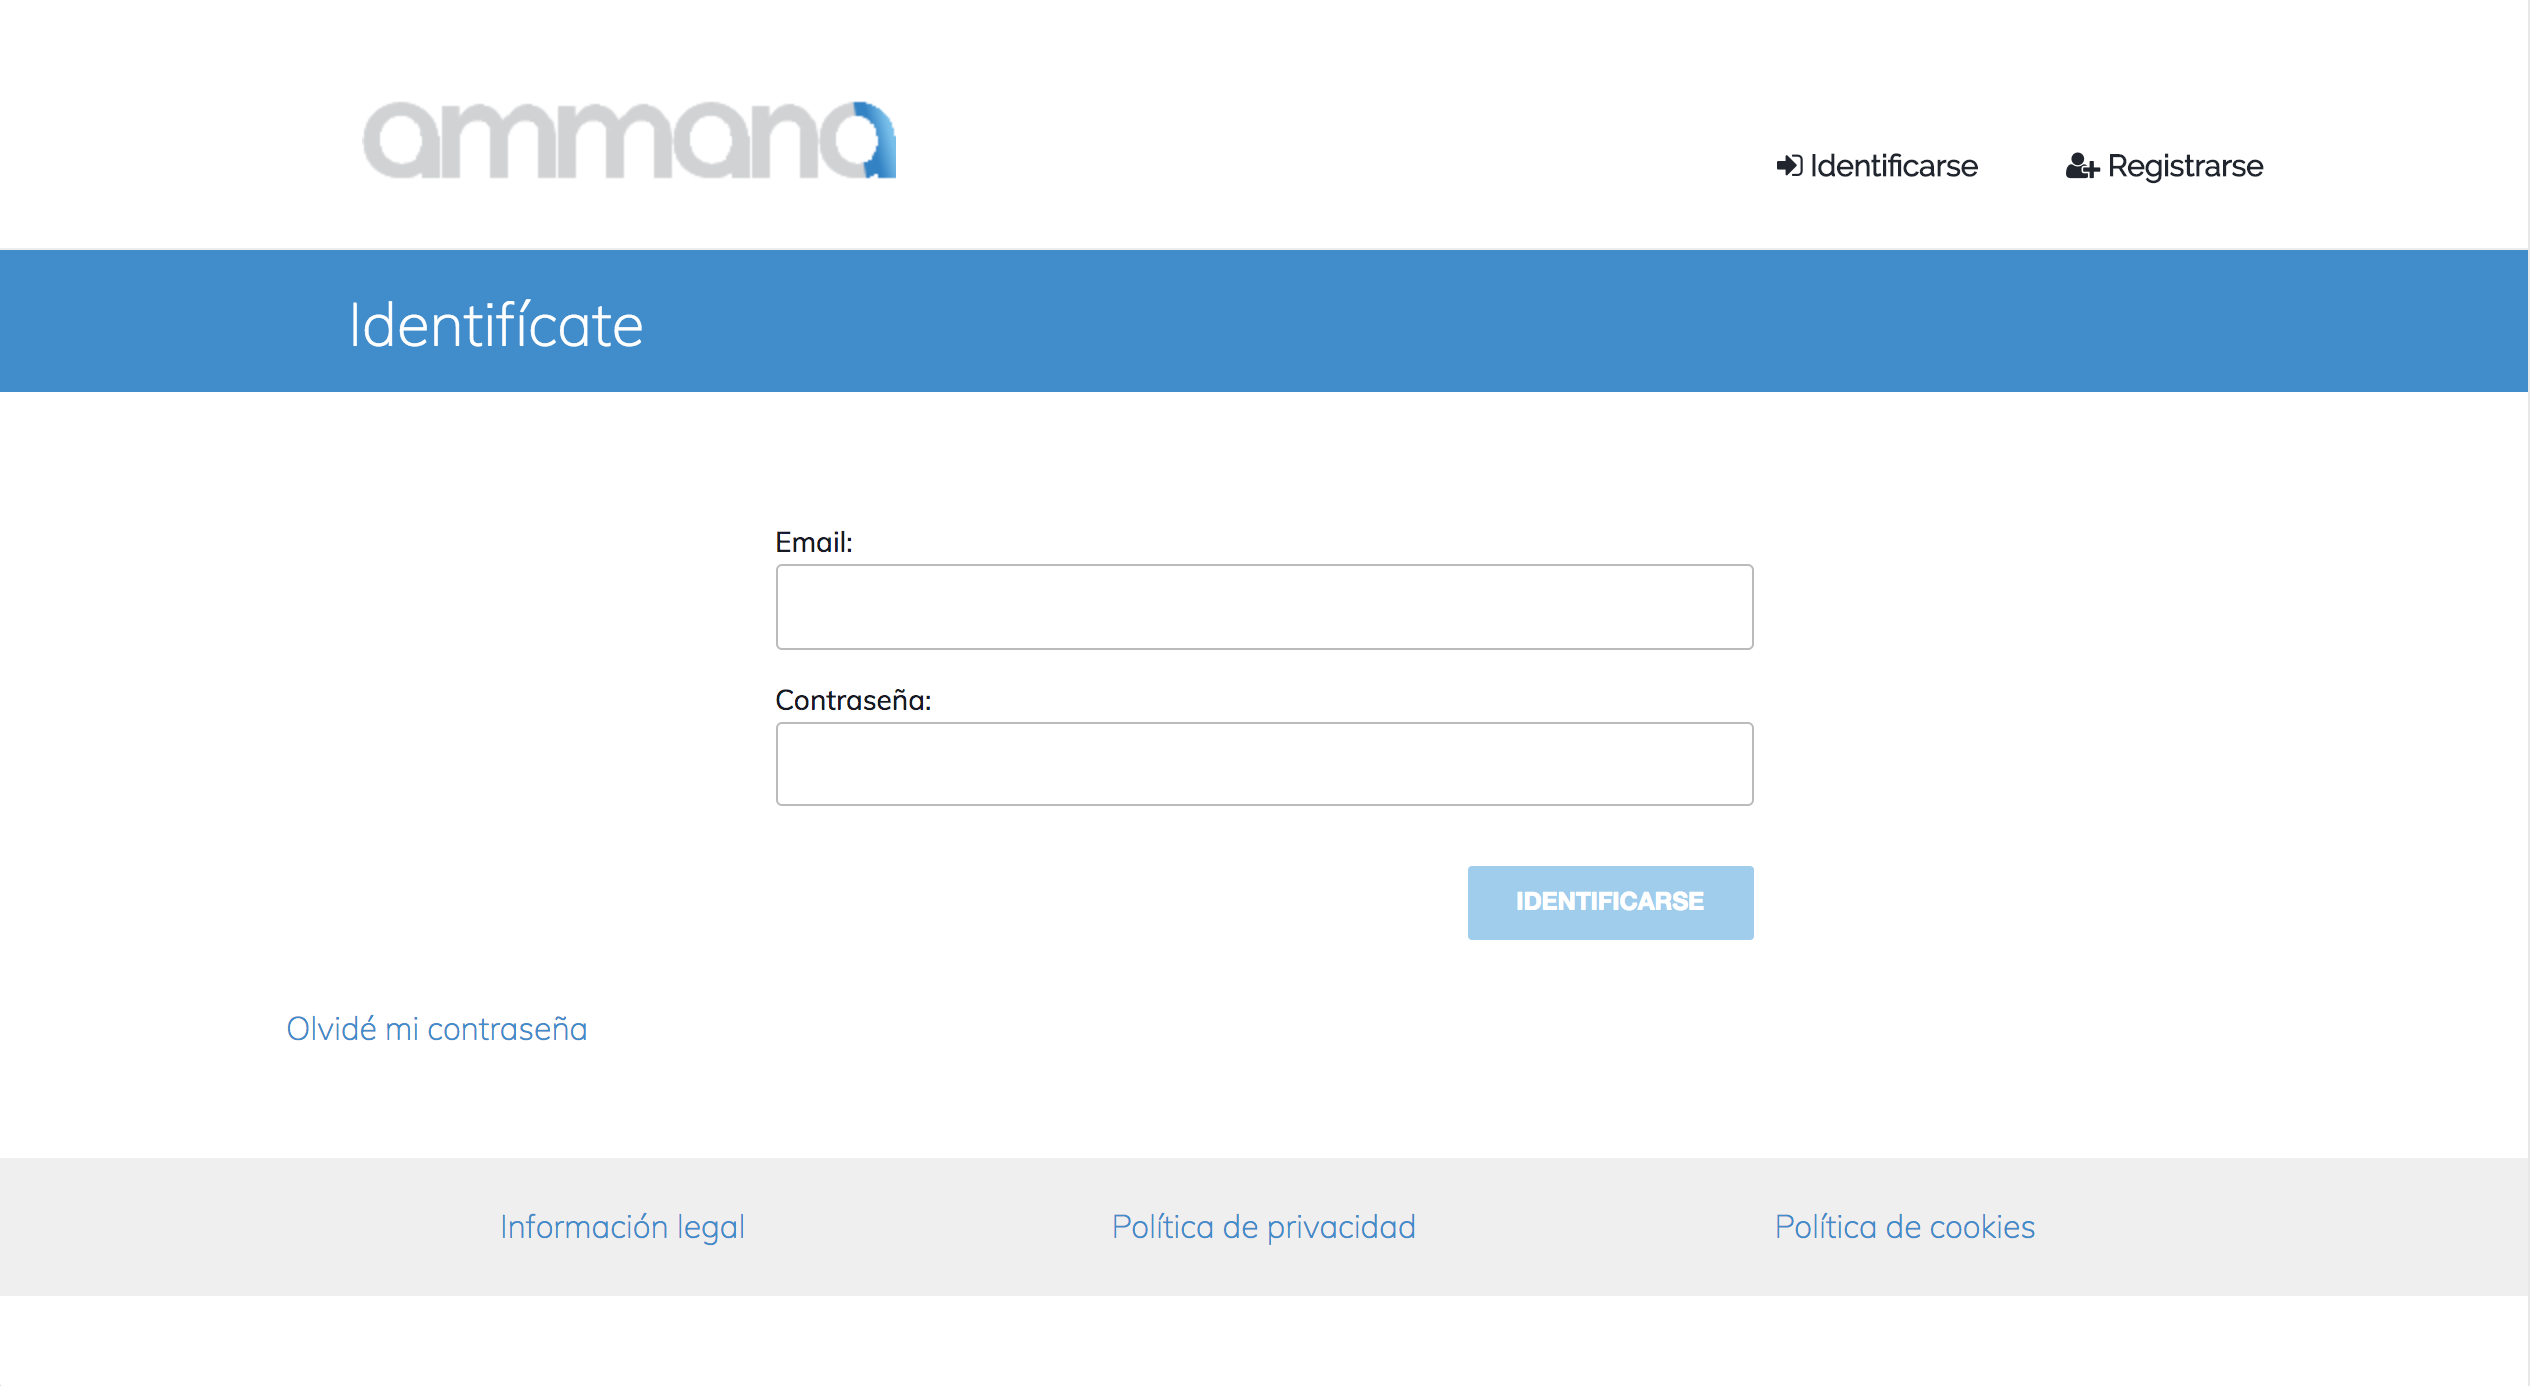
\includegraphics[width=1\linewidth]{login_form.png}%
        }
    \end{minipage}
\end{steps}

%------------------------------------------------

\subsection{Subsection 2} % Sub-section

\lipsum[2] % Dummy text

%------------------------------------------------

\subsubsection{Subsubsection 1} % Sub-sub-section

\lipsum[3] % Dummy text

\begin{figure}[H] % Example image
\center{
\includegraphics[width=0.5\linewidth]{placeholder}}
\caption{Example image.}
\label{fig:speciation}
\end{figure}

%------------------------------------------------

\subsubsection{Subsubsection 2} % Sub-sub-section

\lipsum[4] % Dummy text

%----------------------------------------------------------------------------------------
%	MAJOR SECTION 1
%----------------------------------------------------------------------------------------

\section{Content Section} % Major section

\lipsum[5] % Dummy text

%------------------------------------------------

\subsection{Subsection 1} % Sub-section

\subsubsection{Subsubsection 1} % Sub-sub-section

\lipsum[6] % Dummy text

%------------------------------------------------

\subsubsection{Subsubsection 2} % Sub-sub-section

\lipsum[6] % Dummy text
\begin{wrapfigure}{l}{0.4\textwidth} % Inline image example
  \begin{center}
    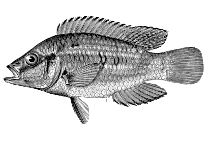
\includegraphics[width=0.38\textwidth]{fish}
  \end{center}
  \caption{Fish}
\end{wrapfigure}
\lipsum[7-8] % Dummy text

%------------------------------------------------

\subsubsection{Subsubsection 3} % Sub-sub-section

\begin{description} % Numbered list example

\item[First] \hfill \\
\lipsum[9] % Dummy text

\item[Second] \hfill \\
\lipsum[10] % Dummy text

\item[Third] \hfill \\
\lipsum[11] % Dummy text

\end{description} 

%----------------------------------------------------------------------------------------
%	MAJOR SECTION X - TEMPLATE - UNCOMMENT AND FILL IN
%----------------------------------------------------------------------------------------

%\section{Content Section}

%\subsection{Subsection 1} % Sub-section

% Content

%------------------------------------------------

%\subsection{Subsection 2} % Sub-section

% Content

%----------------------------------------------------------------------------------------
%	CONCLUSION
%----------------------------------------------------------------------------------------

\section{Conclusion} % Major section

\lipsum[12-13]

%----------------------------------------------------------------------------------------
%	BIBLIOGRAPHY
%----------------------------------------------------------------------------------------

\begin{thebibliography}{99} % Bibliography - this is intentionally simple in this template

\bibitem[Figueredo and Wolf, 2009]{Figueredo:2009dg}
Figueredo, A.~J. and Wolf, P. S.~A. (2009).
\newblock Assortative pairing and life history strategy - a cross-cultural
  study.
\newblock {\em Human Nature}, 20:317--330.
 
\end{thebibliography}

%----------------------------------------------------------------------------------------

\end{document}
